%%%% Semesterprojekt rapport gruppe 2 %%%%
%%%% Elektronik Q1/Q2 2016 %%%%

% Kan anvendes til journaler eller afleveringer
\documentclass[11pt, a4paper, twoside, openany]{memoir}

\usepackage[utf8]{inputenc}		% Dansk input encoding (tegn)
\usepackage[danish]{babel}		% Danske formuleringer / orddeling
\usepackage[T1]{fontenc}		% Output-indkodning af tegnsaet (T1)


%%% Memoir indstillinger
%% Afstand mellem afsnit og videre
%% NIX PILLE - medmindre strengt nødvendigt
\setaftersubsubsecskip{6pt}	
\setbeforesubsubsecskip{6pt}
%\setaftersubsecskip{6pt}
%\setbeforesubsecskip{-\baselineskip}
%\setaftersecskip{6pt}
%\setbeforesecskip{-\baselineskip}
%\setaftersecskip{1ex}

\raggedbottom



\chapterstyle{section}
\usepackage{url}

% ¤¤ Marginer ¤¤ %
\setlrmarginsandblock{3.5cm}{2.5cm}{*}		% \setlrmarginsandblock{Indbinding}{Kant}{Ratio}
\setulmarginsandblock{3.0cm}{2.5cm}{*}		% \setulmarginsandblock{Top}{Bund}{Ratio}
\checkandfixthelayout

%%% Font valg %%%
\usepackage{mathpazo}	%Palatinofont - matematikformler
\usepackage{eulervm}		%Palatinofont

%%% FIGURER OG TABELLER %%%
\usepackage{graphicx} 						% Haandtering af eksterne billeder (JPG, PNG, PDF)

\usepackage[export]{adjustbox}

\usepackage{multirow}                		% Fletning af raekker og kolonner (\multicolumn og \multirow)
\usepackage{colortbl} 						% Farver i tabeller (fx \columncolor, \rowcolor og \cellcolor)
\usepackage[dvipsnames]{xcolor}				% Definer farver med \definecolor. Se mere: http://en.wikibooks.org/wiki/LaTeX/Colors
%\usepackage{flafter}						% Soerger for at floats ikke optraeder i teksten foer deres erence
\usepackage{float}							% Muliggoer eksakt placering af floats, f.eks. \begin{figure}[H]
\usepackage{multicol}         	        	% Muliggoer tekst i spalter
%\usepackage{rotating}						% Rotation af tekst med \begin{sideways}...\end{sideways}
\usepackage{booktabs}
\usepackage{bigstrut}	% Excel2latex måskeh
\usepackage{tabularx}
\usepackage{subfig}

%%% ¤¤ Matematik mm. %%%
\usepackage{amsmath,amssymb,stmaryrd} 		% Avancerede matematik-udvidelser
\usepackage{mathtools}						% Andre matematik- og tegnudvidelser
\usepackage{textcomp}                 		% Symbol-udvidelser (f.eks. promille-tegn med \textperthousand )
\usepackage{siunitx}						% Flot og konsistent praesentation af tal og enheder med \si{enhed} og \SI{tal}{enhed}
\sisetup{output-decimal-marker = {,}}		% Opsaetning af \SI (DE for komma som decimalseparator) 
\sisetup{exponent-product=\cdot, output-product=\cdot}	%Eksponent er gange tegn, output produkt er gange tegn
\sisetup{digitsep = none}					%Almindeligt komma - ingen mellemrum aka. til eurokomma

%%% REFERENCER %%%


%%% MISC %%%
\usepackage{listings}						% Placer kildekode i dokumentet med \begin{lstlisting}...\end{lstlisting}
\definecolor{bg}{HTML}{F0F0F0}
\lstset{language=C++,
				showstringspaces = false,
				backgroundcolor = \color{bg},
                basicstyle=\ttfamily,
                keywordstyle=\color{blue}\ttfamily,
                stringstyle=\color{red}\ttfamily,
                commentstyle=\color{green}\ttfamily,
                morecomment=[l][\color{magenta}]{\#},
                extendedchars=true,
                numbers=left, numberstyle=\tiny,		% Linjenumre
                columns=flexible,						% Kolonnejustering
                breaklines, breakatwhitespace=true,		% Bryd lange linjer
                literate=%
                {æ}{{\ae}}1
                {å}{{\aa}}1
                {ø}{{\o}}1
                {Æ}{{\AE}}1
                {Å}{{\AA}}1
                {Ø}{{\O}}1
}


\usepackage{lipsum}							% Dummy text \lipsum[..]
\usepackage[shortlabels]{enumitem}			% Muliggoer enkelt konfiguration af lister
\usepackage{pdfpages}						% Goer det muligt at inkludere pdf-dokumenter med kommandoen \includepdf[pages={x-y}]{fil.pdf}	
\pdfoptionpdfminorversion=6					% Muliggoer inkludering af pdf dokumenter, af version 1.6 og hoejere

%	¤¤ Afsnitsformatering ¤¤ %
%\setlength{\parindent}{0mm}           		% Stoerrelse af indryk
\setlength{\parskip}{1.5mm}          		% Afstand mellem afsnit ved brug af double Enter
\linespread{1,1}							% Linie afstand

\usepackage{tikz}


% ¤¤ Visuelle  ¤¤ %
\usepackage[colorlinks]{hyperref}			% Danner klikbare referencer (hyperlinks) i dokumentet.
\hypersetup{colorlinks = true,				% Opsaetning af farvede hyperlinks (interne links, citeringer og URL)
	linkcolor = black,
	citecolor = black,
	urlcolor = black
}



%%% Referencer / Bibliografi %%%
%\usepackage[backend=biber, sorting=none, style=numeric]{biblatex}
%\bibliography{../referencer.bib}


\usepackage[draft, danish]{fixme}
\fxsetup{layout=footnote}

\graphicspath{{../fig/}{../fig}{./}}


\usepackage{rotating}
\usepackage{titlesec}

\setcounter{secnumdepth}{4}

\titleformat{\paragraph}
{\normalfont\normalsize\bfseries}{\theparagraph}{1em}{}
\titlespacing*{\paragraph}
{0pt}{3.25ex plus 1ex minus .2ex}{1.5ex plus .2ex}


%%%% Opsætning af dokument %%%%
\newcommand{\forfatter}{Gruppe 2}
\newcommand{\fag}{INDSÆT KURSUS HER}
\newcommand{\titel}{Semesterprojekt 4 Dokumentation}
\date{}

\author{\forfatter}
\title{\titel}

\setlength{\beforechapskip}{10pt}
\setlength{\afterchapskip}{10pt}
% TODO: Skift kapitel header layout
\begin{document}
%\maketitle
\begin{titlingpage}
%\thispagestyle{title}
		
		\begin{center}
				{\huge\bfseries Projekt Universal Actuator Drive}\\
				\vspace{10pt}
				
				{\Huge\bfseries Dokumentation}\\
				
				\vspace{20pt}
				
				{Diplomingeniør Elektronik}\\
				{\large Bachelorprojekt efterår 2017}\\
				
				\vspace{10pt}
				
				Ingeniørhøjskolen Aarhus Universitet\\
				Vejleder: Arne Justesen
				\vspace{10pt}
				
				19. december 2017
				\vspace{10pt}

				\vspace{50pt}
				\begin{minipage}{0.25\linewidth}
					\centering
					\hrule
					\vspace{12pt}
					Nicolai H. Fransen\\
					Studienr. 201404672
				\end{minipage}
				\hspace{10pt}
				\begin{minipage}{0.25\linewidth}
					\centering
					\hrule
					\vspace{12pt}
					Jesper Kloster\\
					Studienr. 201404571
				\end{minipage}
				\hspace{10pt}
		\end{center}
		
		\clearpage
		
	\setcounter{tocdepth}{2}
	\tableofcontents
	\clearpage
	
	%\include{tex/indledning/indledning}
	
	\chapter{Kravspecifikation}

%\subsection{Prioritering / Afgrænsning} måske?
%Moscow
Kravene til produktet er prioriteret ved brug af MoSCoW metoden. Her er kravene for produktet inddelt i fire kategorier, hvor de vigtigste elementer er prioriteret højest. \textbf{Must} benævner de krav som er vigtigst at opfylde, og som er absolut nødvendigt for produktet. \textbf{Should} er de krav produktet bør opfylde. \textbf{Could} er kravene som produktet evt. kunne opfylde, hvis projektets tidsramme tillader det. \textbf{Won't} er krav som ikke vil blive opfyldt inden for projektets tidsrammer, men evt. kan tages med i senere iterationer.

\noindent Følgende opdeling viser kravene udvalgt for dette projekt:
\begin{itemize}
	\item[\textbf{Must}]
		\begin{itemize}
			\item Holde konstant udgangsstrøm og -spænding
			\item Have stabil regulering
			\item Ikke påvirke andre moduler ved fejl
			\item Konstrueres med EEE komponenter

		\end{itemize}
	\item[\textbf{Should}]
		\begin{itemize}
			\item Have programmerbar udgangsstrøm og -spænding

		\end{itemize}
	\item[\textbf{Could}] 
		\begin{itemize}
			\item Have overstrømsbeskyttelse på udgangen

		\end{itemize}
	\item[\textbf{Won't}]
		\begin{itemize}
			\item Indeholde galvanisk adskillelse
		\end{itemize}
\end{itemize}
% De krav der er kritisk for selve funktionen af bilen, dvs. bevægelse / styring, er prioriteret højest. Herefter er krav, som afhænger af bla bla bla. Måske.

\begin{figure}[H]
	\centering
	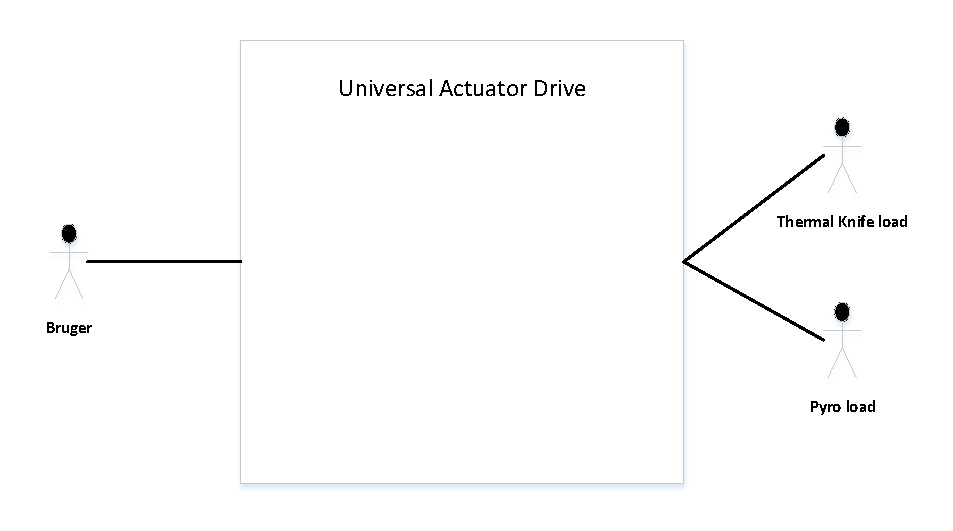
\includegraphics{tex/Kravspecifikation/billeder/AktorkontekstdiagramV1.pdf}
	\caption{Aktør-kontekst diagram}
\end{figure}

\begin{figure}[H]
	\centering
	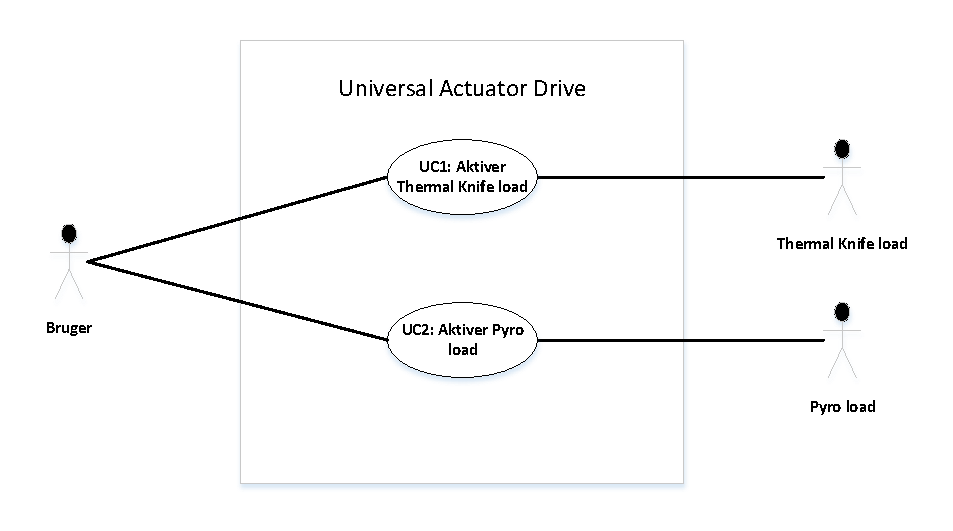
\includegraphics{tex/Kravspecifikation/billeder/UseCasediagramV1.pdf}
	\caption{Use case diagram}
\end{figure}

\section{Aktørbeskrivelse}
I det følgende afsnit beskrives systemets aktører. Ved hver aktør angives typen, samt en kort beskrivelse af aktørens funktion og/eller hvordan de påvirker systemet.

\begin{framed}
	\subsection{Aktør: Bruger}
	\subsubsection*{Type:}
		Primær
	
	\subsubsection*{Beskrivelse:}
		Brugeren interagerer med systemet, ved at indstille den ønskede load type.
\end{framed}

\begin{framed}
	\subsection{Aktør: Thermal Knife load}
	\subsubsection*{Type:}
	Sekundær
	
	\subsubsection*{Beskrivelse:}
	Thermal Knife load er en load type
\end{framed}

\begin{framed}
	\subsection{Aktør: Pyro load}
	\subsubsection*{Type:}
	Sekundær
	
	\subsubsection*{Beskrivelse:}
	Pyro load er en load type
\end{framed}

\clearpage


\section{Fully dressed use cases}

\begin{framed}
	\subsection{Use case 1 - Start bil}
	\subsubsection*{Mål:}
		Initiere bilen så den er klar til kørsel og er klar til at modtage input
		
	\subsubsection*{Initiering:}
		Brugeren
	
	\subsubsection*{Aktører:}
		Brugeren (primær)
	
	\subsubsection*{Referencer:}
		Ingen
	
	\subsubsection*{Samtidige forekomster:}
		En
	
	\subsubsection*{Forudsætning:}
		Bilen er slukket og der er forbindelse fra interface til bil
	
	\subsubsection*{Resultat:}
		Bilens sensorer er tændt, motorer er klar, bilen holder stille
	
	\subsubsection*{Hovedscenarie:}
		\begin{enumerate}
			\item Brugeren vælger via interface ''Start bil''
			\item Bilen monitorerer sensorinputs og rapporterer status 
			\item Bilen udfører motortjek ved at køre bilen lidt frem og derefter tilbage
			\item Bilen rapporterer status
			\item Bilen tænder for- og baglys, blinker med blinklys hvis status er OK 
			\begin{description}
					\item[Extension 1:] Status ikke OK
			\end{description}
			\item Bilen afventer brugerinput
		\end{enumerate}
	
	\subsubsection*{Extensions:}
	\textbf{Extension 1:} Status ikke OK	% Fix layout
		\begin{enumerate}
			\item Bilen rapporterer fejl og forsøger at angive hvilken sensor og/eller motor der fejler
		\end{enumerate}
	
\end{framed}
	

% Skabelon
%\begin{framed}
%\subsubsection{Mål:}
%
%\subsubsection{Initiering:}
%
%\subsubsection{Aktører:}
%
%\subsubsection{Referencer:}
%
%\subsubsection{Samtidige forekomster:}
%
%\subsubsection{Forudsætning:}
%
%\subsubsection{Resultat:}
%
%\subsubsection{Hovedscenarie:}
%
%\subsubsection{Extension:}

\section{Ikke-funktionelle krav}
I dette afsnit beskrives de ikke-funktionelle krav. Her opstilles f.eks. krav om præcision, brugervenlighed samt produktets dimensioner.
\begin{itemize}
			\item Inputspændingen skal være mellem 26-100V
			\item Der må maksimalt trækkes en peak-strøm fra inputkilden på 150\% af inputstrømmen
			\item Skal opretholde en outputspænding på op til 21V ved 2,5A
			\item Der må maksimalt være en ripple-spænding på 50mV pk-pk ved fundamental ripple frekvens
			\item Der må maksimalt være switching spikes på 100mV pk-pk
			\item Skal kunne omsætte op til 75W
			\item Skal operere med et tab på maksimalt 5W %%FIXME
			\item Skal implementeres i et volumen mindre end 17x75x100mm på forsiden af PCB, samt 3x75x100mm på bagsiden PCB'et
			\item Skal kunne operere med en omgivelsestemperatur mellem -35\degreeCelsius  og 65\degreeCelsius
			\item Skal have stabil regulering med 10dB gain og 50 graders fasemargin ved:
				\begin{description}
					\item 21V/2A ved høj og lav indgangsspænding
					\item 5A/2\ohm ved høj og lav indgangsspænding
				\end{description}
			\item Reguleringen skal have en risetime på maksimalt 0,5ms uden overshoot
					
\end{itemize}

	
	\chapter{Accepttest}


%% Skabelon
%\begin{table}[H] 			
%	\centering
%	\begin{tabularx}{\textwidth}{|c|X|X|X|X|}
%		\hline
%		\bfseries Use case under test & \multicolumn{4}{|c|}{< Use case >} \\ \hline
%		\bfseries Scenarie & \multicolumn{4}{| c |}{< Scenarie >} \\ \hline
%		\bfseries Prækondition &  \multicolumn{4}{|c|}{< Prækondition >} \\  \hline
%		\bfseries Step  & \bfseries Handling &  \bfseries Forventet & \bfseries Faktisk & \bfseries Vurdering \\ \hline 
%		\end{tabularx}
%		\caption{< Caption >}
%\end{table}

\section{Tests}
\begin{table}[H] 			
	\centering
	\begin{tabularx}{\textwidth}{|c|X|X|X|X|}
		\hline
		\bfseries Use case under test & \multicolumn{4}{|c|}{Use case 1 - Aktiver Thermal Knife load} \\ \hline
		\bfseries Scenarie & \multicolumn{4}{| c |}{Hovedscenarie} \\ \hline
		\bfseries Prækondition &  \multicolumn{4}{|c|}{Hverken Use case 1 eller Use case 2 er under udførelse} \\  \hline
		\bfseries Step  & \bfseries Handling &  \bfseries Forventet & \bfseries Faktisk & \bfseries Vurdering \\ \hline 
		1 & Brugeren vælger Thermal Knife load & Reb bliver brændt over & & \\ \hline
	\end{tabularx}
	\caption{Test for Use case 1 - Aktiver Thermal Knife load - Hovedscenarie}
\end{table}

\begin{table}[H] 			
	\centering
	\begin{tabularx}{\textwidth}{|c|X|X|X|X|}
		\hline
		\bfseries Use case under test & \multicolumn{4}{|c|}{Use case 2 - Aktiver Pyro load} \\ \hline
		\bfseries Scenarie & \multicolumn{4}{| c |}{Hovedscenarie} \\ \hline
		\bfseries Prækondition &  \multicolumn{4}{|c|}{Hverken Use case 1 eller Use case 2 er under udførelse} \\  \hline
		\bfseries Step  & \bfseries Handling &  \bfseries Forventet & \bfseries Faktisk & \bfseries Vurdering \\ \hline 
		1 & Brugeren vælger Pyro load & Krudtladning bliver antændt & & \\ \hline
	\end{tabularx}
	\caption{Test for Use case 2 - Aktiver Pyro load - Hovedscenarie}
\end{table}




\subsection{Test af ikke-funktionelle krav}

\begin{tabularx}{\textwidth}{|X|X|X|X|X|}
	\hline
	\textbf{Krav} & \textbf{Test} & \textbf{Forventet resultat} & \textbf{Resultat} & \textbf{Vurdering} \\ \hline
	Converterens inputspændingen skal være mellem 26-50V & Indgangs-spændingen måles med et voltmeter & Indgangs-spændingen er mellem 26-50V && \\ \hline
	Converteren må maksimalt trække en peak-strøm fra inputkilden på 150\% af DC inputstrømmen & Udgangen belastes af en 3\ohm\ modstand, og der måles strøm på indgangen med oscilloskop & Peak-strømmen overstiger ikke 150\% af DC strømmen & & \\ \hline
	Converteren skal opretholde en outputspænding på 21V $\pm$2\% ved 2,5A $\pm$5\% & Der indsættes en load på 5\ohm\ og udgangs-strøm og -spænding måles med oscilloskop & Spændingen ligger på 12,5V $\pm$2\% og strømmen på 2,5A $\pm$5\% && \\ \hline
	Skal opretholde en outputstrøm op til 5A $\pm$5\% ved 15V $\pm$2\% & Der indsættes en load på 5\ohm\ og udgangs-strøm og -spænding måles med oscilloskop & Spændingen ligger på 15V $\pm$2\% og strømmen på 3A $\pm$5\% && \\ \hline
	Der må maksimalt være en ripple-spænding på 50mV pk-pk & Der indsættes en load på 3\ohm\ og pk-pk måles med oscilloskop & Ripple-spændingen er under 50mV pk-pk && \\ \hline
	Der må maksimalt være switching spikes på 100mV pk-pk &  &  && \\ \hline
	Skal kunne omsætte op til 75W & Der indsættes en load på 3\ohm\ og der måles på oscilloskopet om der holdes en spænding på 15V $\pm$2\% samt en strøm på 5A $\pm$5\% & Der måles en spænding på 15V $\pm$2\% samt en strøm på 5A $\pm$5\% hvilket giver 75W && \\ \hline
\end{tabularx}



\begin{tabularx}{\textwidth}{|X|X|X|X|X|}
	\hline
	\textbf{Krav} & \textbf{Test} & \textbf{Forventet resultat} & \textbf{Resultat} & \textbf{Vurdering} \\ \hline
	Skal operere med et tab på maksimalt 5W & Der indsættes en load på 3\ohm\ Indgangs-spænding og strøm måles og omregnes til effekt. Det samme gøres for udgangs-spænding og -strøm. & De 2 effekter trukket fra hinanden giver maksimalt 5W && \\ \hline 
	Skal implementeres i et volumen mindre end 17x75x100mm på forsiden af PCB'et, samt 3x75x100mm på bagsiden af PCB'et & Med målebånd måles dimensionerne af PCB'et først på forsiden og derefter på bagsiden. & Dimensionerne overskrider ikke 17x75x100mm på forsiden af PCB'et og 3x75x100mm på bagsiden af PCB'et && \\ \hline
	Skal kunne operere med en omgivelsestemperatur mellem -35\degreeCelsius\ og 65\degreeCelsius\ & Der indsættes en load på 3\ohm\ og der måles på oscilloskopet om der holdes en spænding på 15V $\pm$2\% samt en strøm på 5A $\pm$5\%. Først testes ved -35\degreeCelsius\ og derefter ved 65\degreeCelsius\ & Der måles en spænding på 15V $\pm$2\% samt en strøm på 5A $\pm$5\% hvilket giver 75W ved begge temperature && \\ \hline

\end{tabularx}



\begin{tabularx}{\textwidth}{|X|X|X|X|X|}
	\hline
	\textbf{Krav} & \textbf{Test} & \textbf{Forventet resultat} & \textbf{Resultat} & \textbf{Vurdering} \\ \hline
	Skal have stabil regulering med 10dB gain og 50 graders fasemargin ved 21V/2,5A ved en indgangsspænding på 26V og 100V & Først indstilles indgangsspændingen til 26V og vha. oscilloskopets network analyser genereres et bodeplot ved at måle over loaden. Dette gentages med en indgangsspænding på 100V & På bodeplottet ses en stabil regulering med 10dB gain og 50 graders fase margin for både 26V og 100V && \\ \hline
	Skal have stabil regulering med 10dB gain og 50 graders fasemargin ved 5A/3\ohm\ ved en indgangsspænding på 26V og 100V & Først indstilles indgangsspændingen til 26V og vha. oscilloskopets network analyser genereres et bodeplot ved at måle over loaden. Dette gentages med en indgangsspænding på 100V & På bodeplottet ses en stabil regulering med 10dB gain og 50 graders fase margin for både 26V og 100V && \\ \hline
	Reguleringen skal have en risetime på maksimalt 0,5ms & Ved en load på 3\ohm, udgangsstrøm på 5A $\pm$5\% og udgangsspænding på 15V $\pm$2\% måles risetime med et oscilloskop på udgangen ved et step på indgangen & Der måles en risetime på maksimalt 0,5ms && \\ \hline
\end{tabularx}


\begin{tabularx}{\textwidth}{|X|X|X|X|X|}
	\hline
	\textbf{Krav} & \textbf{Test} & \textbf{Forventet resultat} & \textbf{Resultat} & \textbf{Vurdering} \\ \hline
	Reguleringen skal have et overshoot på maksimalt 5\% & Ved en load på 3\ohm, udgangsstrøm på 5A $\pm$5\% og udgangsspænding på 15V $\pm$2\% måles overshoot med et oscilloskop på udgangen ved et step på indgangen & Der måles et overshoot på maksimalt 5\% && \\ \hline
\end{tabularx}
	
	%\chapter{Systemarkitektur}

 
Følgende afsnit indeholder SysML BDD og IBD. BDD'et bruges til at give overblik over  systemets hardware blokke, samt hvilke inputs og outputs hver blok indeholder. IBD'et viser forbindelserne mellem hardware blokkene, samt hvilken vej kommunikationen foregår..


\section{Block Definitions Diagram}
\noindent Figur~\ref{fig: BDD} viser et Block Definitions Diagram (BDD) over systemet. Det er med for, at give det første overblik over systemet -- altså hvad systemet består af.

Systemet består af fire hardware blokke -- et Input filter, et Power-modul, en PWM-forsyning, samt et PWM-modul.
Input filteret bruges til at filtrer støj der kommer fra inputkilden, og sikrer en stabil inputspænding. Derudover skal det også filtrere støjsignaler der kan løbe tilbage til kilden.
Power-modulet består af selve convertertrinet. Det er i denne blok inputspændingen bliver konverteret om til den korrekte udgangsspænding.
PWM-forsyningen står for at forsyne PWM-modulet. Under opstart vil blokken regulere converterens inputspænding ned til den korrekte spænding på 12V. Mens converterens output vil bruges når outputspændingen er tilstrækkelig.
PWM-modulet står for selve reguleringen af converterens output. Dette sker ved at overvåge både outputspændingen, samt peak-strøm i power-modulet, og tilpasse PWM-signalets duty-cycle herefter.   

\begin{figure}[H]
	\centering
	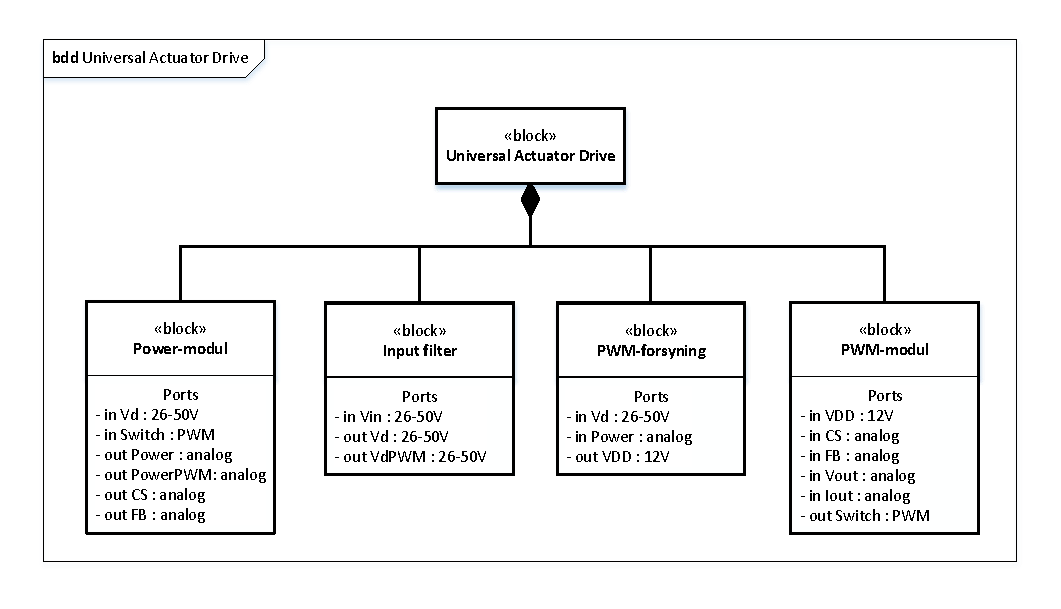
\includegraphics[width=1.00\textwidth]{tex/systemarkitektur/billeder/BDD.pdf}
	\caption{BDD}
	\label{fig: BDD}
\end{figure}

\section{Internal Block Diagram}
\noindent Figur~\ref{fig: IBD} viser et Internal Block Diagram (IBD) over systemet. Dette er skridtet efter BDD'et, og viser hvordan systemets blokke er forbundet.


\begin{figure}[H]
	\centering
	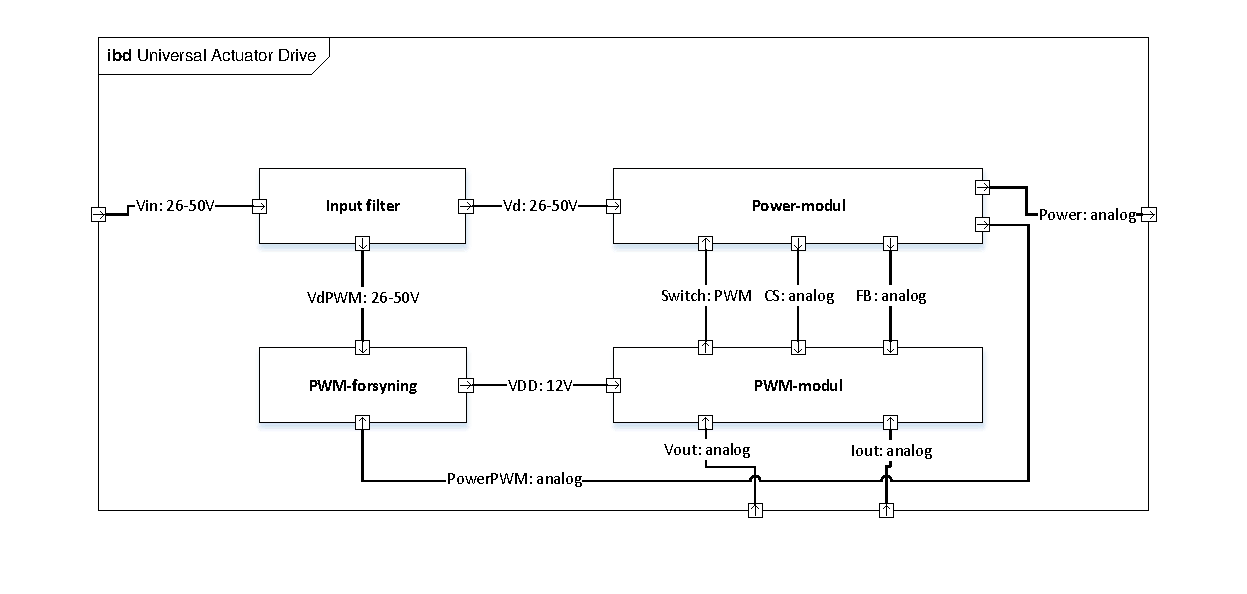
\includegraphics[width=1.00\textwidth]{tex/systemarkitektur/billeder/IBD.pdf}
	\caption{IBD}
	\label{fig: IBD}
\end{figure}


\subsection{Signalbeskrivelse}
\noindent Tabel~\ref*{tabel: Signalbeskrivelse} viser en signalbeskrivelse for systemet. Tabellen indeholder signalets type, navn, og en beskrivelse af signalet.

\begin{table}[htbp]
	\centering
	\begin{tabular}{|l|l|l|}
		\hline
		\textbf{Signal type} 	&\textbf{Navn}		&\textbf{Beskrivelse} \\\hline
		26-50V			&Vin		&Ufiltreret inputspænding på 26-50V\\\hline
		26-50V			&Vd			&filtreret inputspænding på 26-50V\\\hline
		26-50V			&VdPWM			&Input til convertering af PWM-controllerens VDD, under opstart\\\hline
		15-21V			&PowerPWM		&Input til convertering af PWM-controllerens VDD, efter opstart\\\hline
		12V				&VDD		&12V forsyning til PWM-controller\\\hline
		15-21V			&Power		&Converterens outputspænding\\\hline
		PWM				&Switch		&PWM signal til regulering af outputspænding\\\hline
		analog			&CS			&Analogt signal til monitorering af peak-strøm   \\\hline	
		analog			&FB			&Analogt signal til monitorering af outputspænding\\\hline
		Vout			&analog		&0-5V signal, som sætter ønsket udgangsspænding\\\hline
		Iout			&analog		&0-5V signal, som sætter ønsket udgangsstrøm\\\hline
		
	\end{tabular}
	\caption{Signalbeskrivelse}
	\label{tabel: Signalbeskrivelse}
\end{table}


	
	%\include{tex/design/design}

	%\include{tex/Done_acceptest/Done_acceptest}
	
	%\include{<sti/filnavn.tex>}

	
	%%% Foreløbig disposition %%%
	% Forord / indledning
	% Kravspecifikation
	% Systemarkitektur
	%% HW
	%% SW
	% Accepttest
	
%	\printbibliography[title={Litteraturliste}]
	
\end{titlingpage}
\end{document}